%\clearpage
%\subsection{Control Regions (CRs) definitions}
\label{subsec:cr_selection}

In this analysis, we adopt the usual approach for background estimation, combining MC simulations with data-driven methods. Specifically, MC simulations are utilized to model SM background processes, while dedicated Control Regions (CRs) are established to adjust the background normalization within the SRs.

This section will detail the definition of CRs tailored to $W$+jets and \ttbar events. Furthermore, we distinguish between CRs for the resolved and merged categories to address potential discrepancies in background modeling across different \pt ranges.

\subsection{$W$+jets CR (WCR)}

The $W$+jets Control Region (WCR) is defined using mass sidebands relative to the hadronically decaying vector boson in the 1-lepton channel. Notably, in the resolved category, distinct sidebands are identifiable, whereas in the merged category, the definition is more conceptual due to the selection methodology of events. The criteria for event selection in the WCR mirror those in the Signal Region (SR), ensuring analytical consistency. For simplicity, a common sideband is established outside the mass windows of both $W\to qq'$ and $Z \to q\bar{q}$ SRs.
\begin{itemize}
    \item In the resolved category, events must satisfy $50 < m_{jj} < 64$ GeV or $m_{jj} > 106$ GeV, effectively inverting the $m_{jj}$ requirement for SR.
    \item In the merged category, the criterion is failing the high efficiency WP ($\epsilon=80\%$) of the vector boson tagger.
\end{itemize}

Figure \ref{fig:1lep2lepMVHadResCR} shows the sideband distributions in the resolved regions.
%Figure \ref{fig:1lep2lepMVHadMerCR} shows the large-R jet mass distributions in the merged control region. Given that the merged CR is defined by the vector boson tagger's $80\%$ working point, the mass distribution encompasses events within both the sidebands and the mass window.

\begin{figure}[ht]
    \centering
    \begin{subfigure}{0.3\textwidth}
        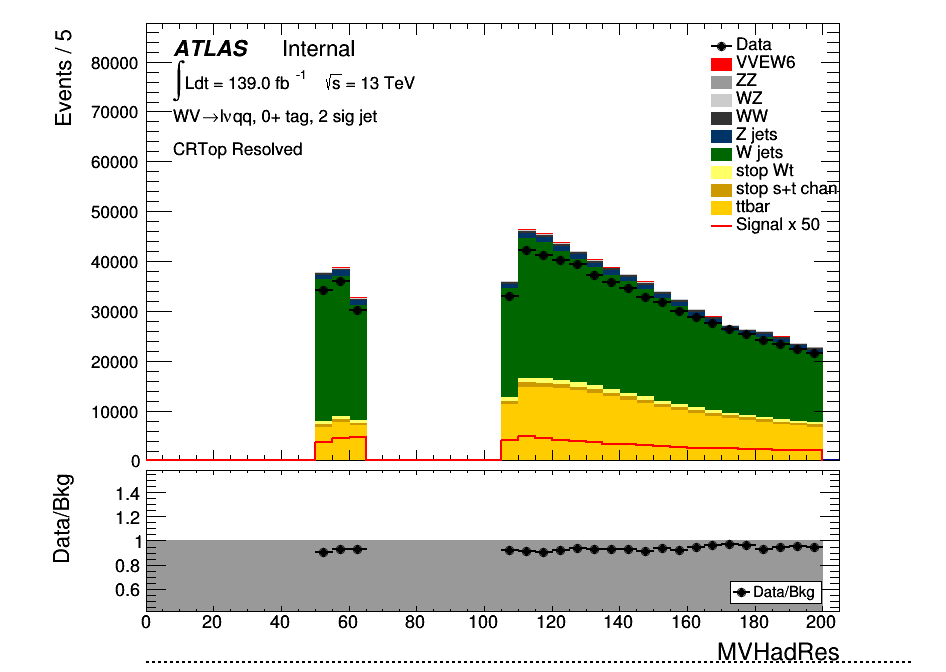
\includegraphics[width=\linewidth]{figures/1lep/CRPlots/C_0ptag2pjet_0ptv_CRVjet_MVHadRes_Lin.png}
        \caption{\emph{\olep, resolved WCR}}
    \end{subfigure}
    \caption{$m_{jj}$ plot in the sidebands.}
    \label{fig:1lep2lepMVHadResCR}
\end{figure}

\clearpage
\subsection{TCR}



The TCR is established by mandating the presence of at least one $b$-tagged jet, as opposed to a $b$-veto. Figure \ref{fig:1lepNBjetsPresel} displays the $b$-jets multiplicity distributions for both the resolved and merged regimes. The TCR's defining feature, the inclusion of additional $b$-jets, creates orthogonal cuts that align with the mass window phase spaces. Consequently, in the merged regime, the TCR adopts the High Purity (HP) and Low Purity (LP) categorization analogous to the SRs.

\begin{figure}[ht]
    \centering
    \begin{subfigure}{0.3\textwidth}
        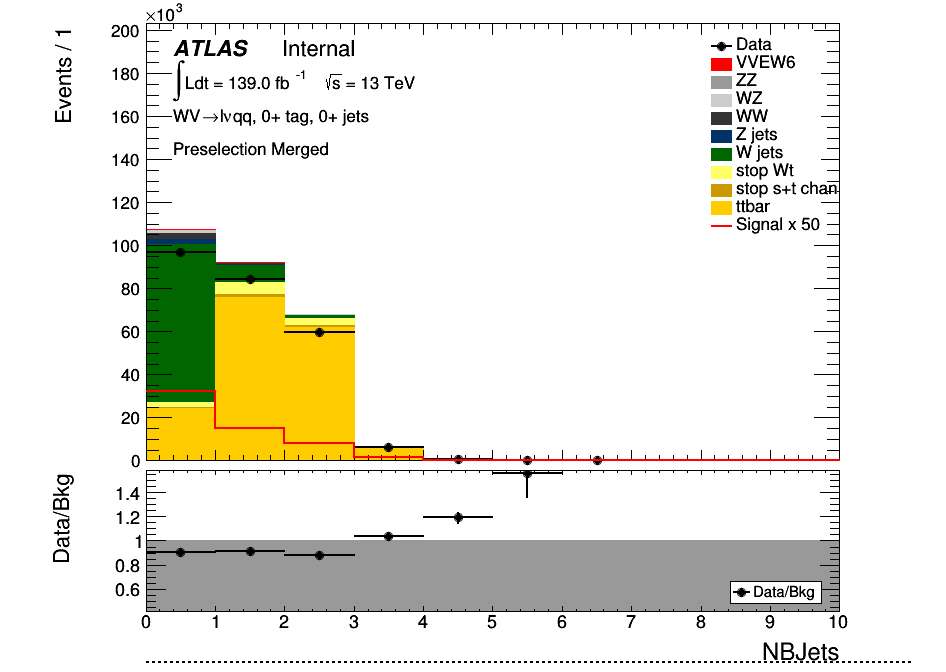
\includegraphics[width=\linewidth]{figures/1lep/CRPlots/C_0ptag0pjet_0ptv_Presel_Merged_NBJets_Lin.png}
        \caption{After merged preselection}
    \end{subfigure}
    \begin{subfigure}{0.3\textwidth}
        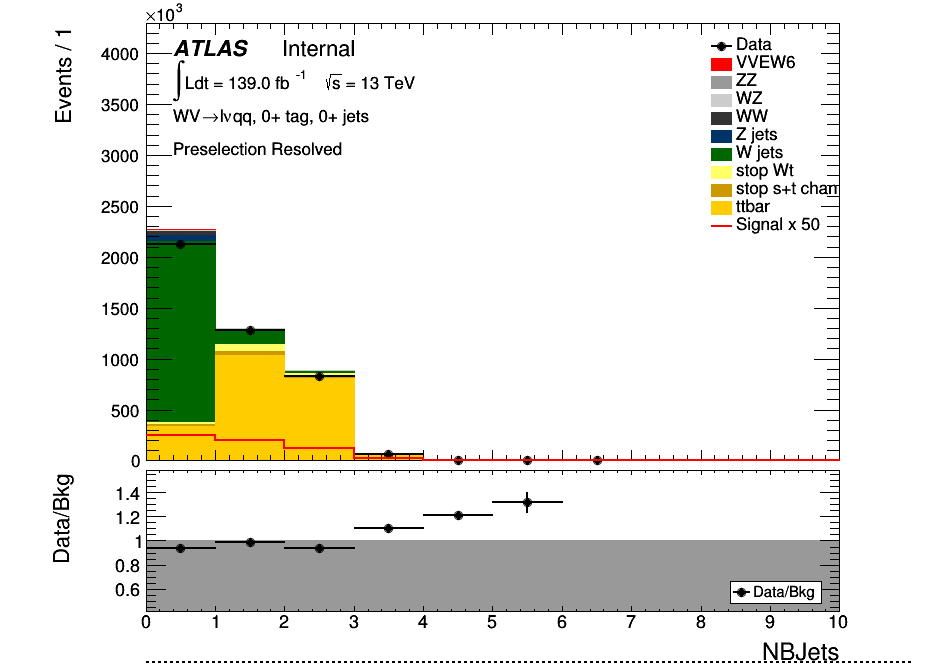
\includegraphics[width=\linewidth]{figures/1lep/CRPlots/C_0ptag0pjet_0ptv_Presel_Resolved_NBJets_Lin.png}
        \caption{After resolved preselection}
    \end{subfigure}
    \caption{Bjets multiplicity in the 1-lepton channel, after common preselection cuts have been applied.}
    \label{fig:1lepNBjetsPresel}
\end{figure}

%%%%%%%%%%%%%%%%%%%%%%%%%%%%%%%%%%%%%%%%%%%%%

%%%We use a combined MC template and data-driven background estimation, indeed, we rely on the MC simulations samples for the SM background processes, but we use dedicated Control Regions (CRs) to constrain the normalization of the background expectation in the SRs.
%%%
%%%The dedicated CRs to the $Z$+jets, $W$+jets and \ttbar events are defined in this section.
%%%
%%%The $Z$+jets, $W$+jets and \ttbar CRs are used in this analysis shared 
%%%across the the 0-, 1- and 2-lepton channels;
%%%for instance, the \ttbar CR is defined using \olep events only, 
%%%and used to constraint this background in all the SRs.
%%%Independent CRs for resolved and merged categories are, instead,
%%%used to account for possible mis-modelling of the background depending on \pt range.
%%%
%%%\subsubsection{$W$+jets CR (WCR) and $Z$+jets CR (ZCR)}
%%%%\textbf{$W$+jets CR (WCR) and $Z$+jets CR (ZCR)}
%%%
%%%The $V$+jets CR (VCR) for $V=W/Z$, $W$+jets CR (WCR), and $Z$+jets CR (ZCR) are defined using the mass sidebands with respect to hadronically decaying vector boson in 0-, 1-, and 2-lepton channels, respectively.
%%%The event selections are otherwise the same as the SR selections.
%%%For the simplicity of the analysis, the common sideband is defined as the outside of both $W\to q\bar{q}$ and $Z \to q\bar{q}$ signal regions.
%%%The same definition is used in all channels:
%%%In the resolved category, a requirement of $50 < m_{jj} < 64$ GeV or $m_{jj} > 106$ GeV is applied which is an inversion of the $m_{jj}$ cut in the corresponding SR.
%%%In the merged case, the event has to fail the vector boson tagger's lower working point of $\epsilon=80\%$.
%%%%In the merged category, the purity of the $W$+jets background is 77\,\% in the lower mass side band, 62\,\% in the higher mass side band region and 65\,\% in total. The $t\bar{t}$ contamination is 30\,\% in higher mass side band regions. 
%%%
%%%Figure \ref{fig:1lep2lepMVHadResCR} shows an example of sideband distributions in the resolved regions.
%%%Figure \ref{fig:1lep2lepMVHadMerCR} shows an example of fat jet mass distributions in the merged control region; 
%%%since the merged CR is defined using the full tagger 80\% WP, the mass distribution collects events both 
%%%in the sidebands both in the mass window.
%%%
%%%\begin{figure}[ht]
%%%    \centering
%%%    \begin{subfigure}{0.3\textwidth}
%%%        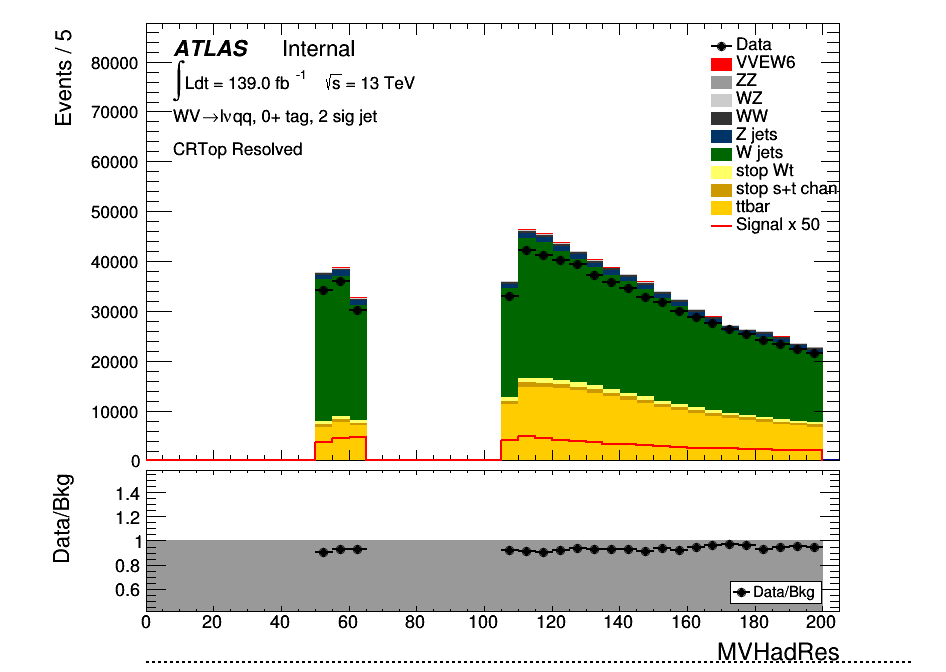
\includegraphics[width=\linewidth]{figures/1lep/CRPlots/C_0ptag2pjet_0ptv_CRVjet_MVHadRes_Lin.png}
%%%        \caption{\emph{\olep, resolved WCR}}
%%%    \end{subfigure}
%%%    % You can add other subcaptions here if needed
%%%    \caption{$m_{jj}$ plot in the sidebands in \zlep channel VCR (a), in \olep WCR (b) and \tlep channel ZCR (right).}
%%%    \label{fig:1lep2lepMVHadResCR}
%%%\end{figure}

%\begin{figure}[ht]
%    \begin{center}
%        \subfigure[]{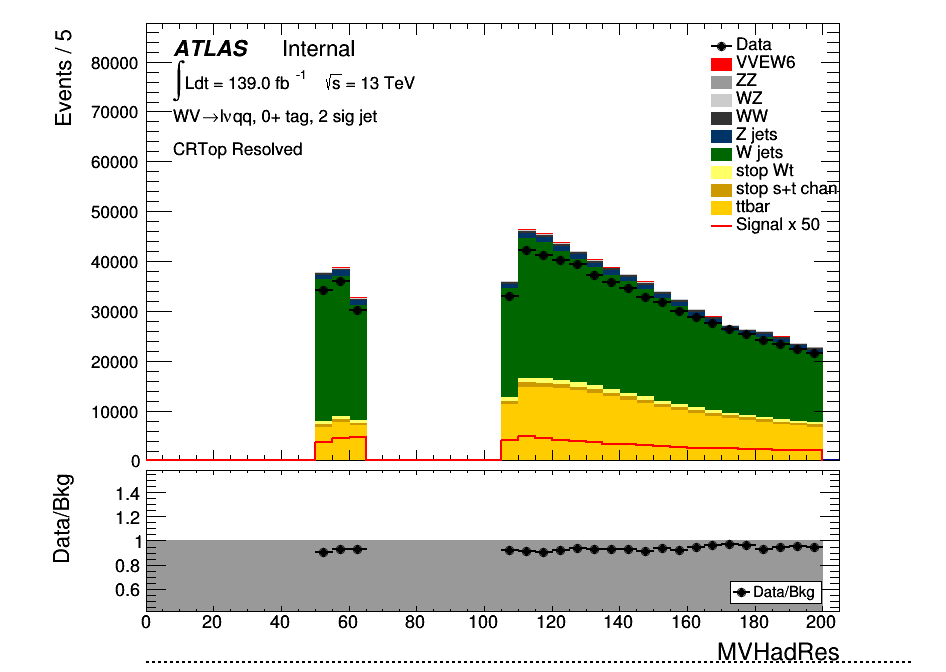
\includegraphics[width=0.3\textwidth]{figures/1lep/CRPlots/C_0ptag2pjet_0ptv_CRVjet_MVHadRes_Lin.png}}
%        \caption{ $m_{jj}$ plot in the sidebands in 1-lepton channel. }
%    \end{center}
%    \label{fig:1lepMVHadResCRVjet}
%\end{figure}

%\subsubsection{$t\bar{t}$ CR (TCR)}
%\textbf{$t\bar{t}$ CR (TCR)}

%Two sets of the \ttbar CR (TR1 and TR2) can be used in this analysis.

%%%In 1-lepton channel, TCR is defined by requiring at least one $b$-tagged jet instead of $b$-veto; distributions of the b-jets multiplicity for both resolved and merged regime are shown in figure \ref{fig:1lepNBjetsPresel}. 
%The purity of the $t\bar{t}$ background in this 
%region is 85\,\%. Signal contamination in both $W$+jets and $t\bar{t}$ control regions is negligible. The purity 
%of $W$+jets in WR is a bit poor, but the simultaneous fit to TR and WR makes it possible to determine the 
%normalization of $W$+jets correctly, thanks to high purity of $t\bar{t}$ in TR.

%%%Since, the orthogonal cut is represented by the additional bjets in the event, 
%%%the TCR correspond to mass window phase spaces, therefore, for the merged regime
%%%TCR inherit the HP and LP splitting as for the SRs.
%%%
%%%\begin{figure}[ht]
%%%    \centering
%%%    \begin{subfigure}{0.3\textwidth}
%%%        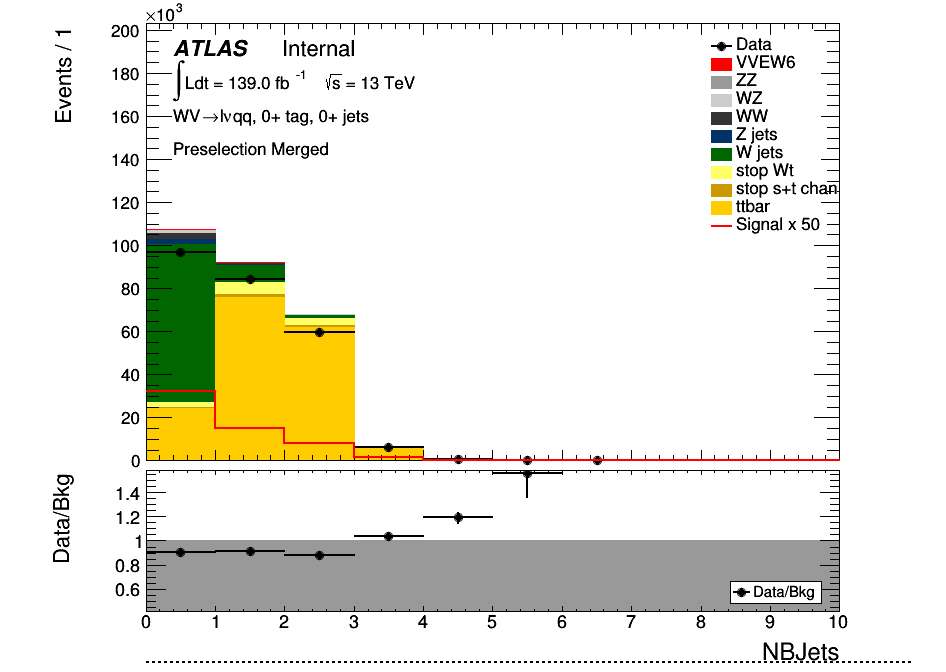
\includegraphics[width=\linewidth]{figures/1lep/CRPlots/C_0ptag0pjet_0ptv_Presel_Merged_NBJets_Lin.png}
%%%        \caption{After merged preselection}
%%%    \end{subfigure}
%%%    \begin{subfigure}{0.3\textwidth}
%%%        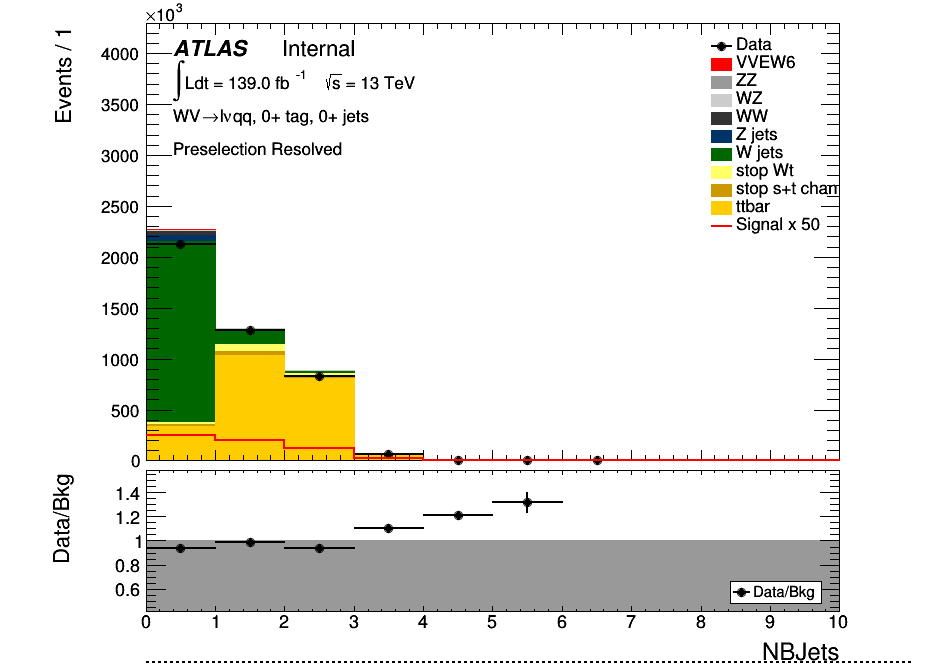
\includegraphics[width=\linewidth]{figures/1lep/CRPlots/C_0ptag0pjet_0ptv_Presel_Resolved_NBJets_Lin.png}
%%%        \caption{After resolved preselection}
%%%    \end{subfigure}
%%%    \caption{Bjets multiplicity in the 1-lepton channel, after common preselection cuts have been applied.}
%%%    \label{fig:1lepNBjetsPresel}
%%%\end{figure}


